\documentclass[11pt, a4paper]{article}
\setlength{\oddsidemargin}{0.5cm}
\setlength{\evensidemargin}{0.5cm}
\setlength{\topmargin}{-1.6cm}
\setlength{\leftmargin}{0.5cm}
\setlength{\rightmargin}{0.5cm}
\setlength{\textheight}{24.00cm} 
\setlength{\textwidth}{15.00cm}
\parindent 0pt
\parskip 5pt
\pagestyle{plain}

\newcommand{\namelistlabel}[1]{\mbox{#1}\hfil}
\newenvironment{namelist}[1]{%1
\begin{list}{}
    {
        \let\makelabel\namelistlabel
        \settowidth{\labelwidth}{#1}
        \setlength{\leftmargin}{1.1\labelwidth}
    }
  }{%1
\end{list}}

\usepackage{graphicx}
\graphicspath{ {../figs/} }
\usepackage{hyperref}
\usepackage{cite}

\begin{document}


\begin{namelist}{xxxxxxxxxxxx}
\item[{\bf Title:}]
    Learning Automata of Black Box Software and Hardware via Side Channel Analysis
\item[{\bf Author:}]
	Johnathan DiMatteo
\item[{\bf Supervisor:}]
	Sebastian Fischmeister
\end{namelist}

\section*{Motivation}
% In this section you should give some background to your
% research area. What is the problem you are tackling, and why is it
% worthwhile solving? Who has already done some work in this area,
% and what have they achieved?

The goal of this paper is to enforce security and safety in these devices through reverse engineering, or \textit{Model Learning}:
automatic algorithms that ``determine in which global states the device can be and which state transitions and outputs occur in response to which inputs'' \cite{vaandrager2017model}.
% ============= MODEL LEARNING ===============%
Our proposed method is to use \textit{Side Channel Analysis} to make learning more ``black box''.
One application of this technology is to verify software and hardware systems conform to design specifications.
Another is to perform this on a live system to see if it has been compromised (i.e. an attacker downloads new firmware onto the device), thus alerting users.

\subsection*{Background}

\textbf{State diagrams} are a way to model a system concerning a finite number of states, inputs and outputs.
\textbf{Inputs} are external stimuli that interact with the system.
\textbf{Outputs} are a system's response to an input.
%============== WHAT IS A STATE? COFFEE MACHINE EXAMPLE ====== %
A \textbf{state} determines the behavior of a system.
For example, a coffee machine can have three states, ``Off'', ``Standby'', and ``Ready''.
The coffee maker will only pour coffee after the press of Button B in the ``Ready'' state, will be turned off in the ``Off'' state, and will wait for the user to load a coffee pod in the ``Standby'' state.
A state is bound to a set of rules and functions (i.e. it is impossible to pour coffee in the ``Off'' state).
State diagrams are common in software validation.
We will be focusing on a specific type of state diagram model known as a Mealy Machine.

%======WHAT IS A STATE DIAGRAM MODEL ========%
% ======= INPUTS? OUTPUTS? ===== %

\begin{figure}[!h]
    \hspace*{2cm}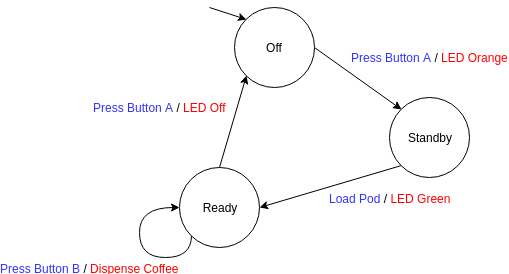
\includegraphics[scale=0.5]{coffee}
    \caption{Example of a simple Mealy Machine for a coffee maker.}
    \label{coffee}
\end{figure}

\section*{Problem Statement} 
%Now state explicitly the hypothesis you aim to
%test. Make references to the items listed in the Reference section
%that back up your arguments for why this is a reasonable
%hypothesis to test, for example the work of Knuth~\cite{knuth}.
%Explain what you expect will be accomplished by undertaking this
%particular project.  Moreover, is it likely to have any other
%applications?
\begin{figure}[!h]
    \centering
    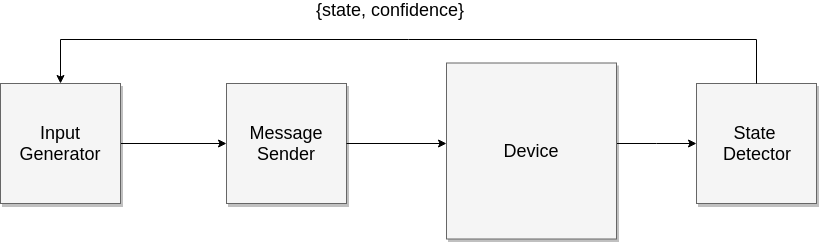
\includegraphics[scale=0.5]{state-detector.png}
    \label{The system under active model learning.}
\end{figure}

\begin{enumerate}
    \item \textbf{Input Generator}: Given the current predicted state (\textbf{output? - ask Sebastian}) and history of previous states (\textbf{outputs?}) and queries, determine the next query that is most likely to induce a state change in the system under observation.
    \item \textbf{State Detector}: Given a response from the system under observation and history of previous responses, estimate the current state (\textbf{output? - ask Sebastian}).
    \item \textbf{Message Sender}: Given a query, translate the query into a valid message accepted by the system.
    %valid inputs to system and outputs from the system to valid inputs to the Learner.
    %the Learner's queries into valid inputs to the system, 
    %and classifying the response of the system to the output alphabet understood by the Learner.
\end{enumerate}

\nocite*{}
\bibliography{bibfile}{}
\bibliographystyle{plain}

\end{document}


